\documentclass[11pt]{article}
\usepackage{amsmath}
\usepackage[margin=1in]{geometry}
\usepackage{tikz} % For TikZ diagrams
\usetikzlibrary{shapes,arrows} % TikZ libraries
\usepackage{graphicx} % Needed for including graphics
\usepackage{listings} % Needed for including code
\usepackage{color} % For coloring code

% Define colors for code listing
\definecolor{codegreen}{rgb}{0,0.6,0}
\definecolor{codegray}{rgb}{0.5,0.5,0.5}
\definecolor{codepurple}{rgb}{0.58,0,0.82}
\definecolor{backcolour}{rgb}{0.95,0.95,0.92}

% Setup the style for the code listing
\lstdefinestyle{mystyle}{
    backgroundcolor=\color{backcolour},   
    commentstyle=\color{codegreen},
    keywordstyle=\color{magenta},
    numberstyle=\tiny\color{codegray},
    stringstyle=\color{codepurple},
    basicstyle=\ttfamily\footnotesize,
    breakatwhitespace=false,         
    breaklines=true,                 
    captionpos=b,                    
    keepspaces=true,                 
    numbers=left,                    
    numbersep=5pt,                  
    showspaces=false,                
    showstringspaces=false,
    showtabs=false,                  
    tabsize=2
}

% Apply the style to the listings package
\lstset{style=mystyle}
% TikZ styles
\tikzstyle{input} = [coordinate]
\tikzstyle{output} = [coordinate]
\tikzstyle{sum} = [draw, circle, node distance=1.5cm, inner sep=6pt]
\tikzstyle{block} = [draw, rectangle, minimum height=2em, minimum width=2.5em]

\begin{document}
\title{ELCT 331 Control Systems Assignment 4}
\author{Jacob C. Vaught}
\date{November 14th, 2023}
\maketitle
\section*{Problem \#1}
The following Forward path Transfer Functions are given:

\begin{flalign}
  (a) \quad G(s) &= \frac{K}{(1+s)(1+10s)(1+20s)} && \notag \\
  (b) \quad G(s) &= \frac{10e^{-0.2s}}{(1+s)(1+10s)(1+20s)} && \notag \\
  (c) \quad G(s) &= \frac{10(s+1)}{s(s+5)(s+6)} && \notag \\
  (d) \quad G(s) &= \frac{100(s-1)}{s^2(s+5)(s+6)^2} && \notag \\
  (e) \quad G(s) &= \frac{10(s+1)}{s^3(s^2 + 5s + 5)} && \notag \\
  (f) \quad G(s) &= \frac{100}{s^3(s+2)^2} && \notag \\
  (g) \quad G(s) &= \frac{5(s+2)}{s^2(s+4)} && \notag \\
  (h) \quad G(s) &= \frac{8(s+1)}{(s^2 + 2s + 3)(s+1)} && \notag
\end{flalign}
\subsection*{Objective}
For the unity-feedback control systems described above, determine the steady-state error for:
\begin{itemize}
  \item A unit-step input
  \item A unit-ramp input
  \item A parabolic input, \( \dfrac{t^2}{2} u_s(t) \)
\end{itemize}
Check the stability of the system before applying the final-value theorem.

\newpage
\subsection*{Solution for (a)}

\textbf{Stability Analysis:}
All poles of \(G(s)\) are negative \((-1, -10, -20)\). Therefore, the system is stable.
\newline
\textbf{Steady-State Error Analysis:}
\newline
\textit{For a unit-step input:}
\[
K_p = \lim_{{s \to 0}} G(s) = K. \quad E_{ss} = \frac{1}{1+K_p} = \frac{1}{1+K}
\]
\textit{For a ramp input:}
\[
K_v = \lim_{{s \to 0}} sG(s) = 0. \quad E_{ss} \text{ is infinite.}
\]
\textit{For a parabolic input:}
\[
K_a = \lim_{{s \to 0}} s^2G(s) = 0. \quad E_{ss} \text{ is infinite.}
\]
\subsection*{Solution for (b)}

\textbf{Stability Analysis:}
All poles of \(G(s)\) are negative \((-1, -10, -20)\). Therefore, the system is stable.
\newline
\textbf{Steady-State Error Analysis:}
\newline
\textit{For a unit-step input:}
\[
K_p = \lim_{{s \to 0}} G(s) = 10. \quad E_{ss} = \frac{1}{1+K_p} = \frac{1}{11}
\]
\textit{For a ramp input:}
\[
K_v = \lim_{{s \to 0}} sG(s) = 0. \quad E_{ss} \text{ is infinite.}
\]
\textit{For a parabolic input:}
\[
K_a = \lim_{{s \to 0}} s^2G(s) = 0. \quad E_{ss} \text{ is infinite.}
\]

\subsection*{Solution for (c)}

\textbf{Stability Analysis:}
The poles of \(G(s)\) are \(s = 0, -5, -6\). One pole is at the origin, and the rest are negative. Therefore, the system is marginally stable.
\newline
\textbf{Steady-State Error Analysis:}
\newline
\textit{For a unit-step input:}
\[
K_p = \lim_{{s \to 0}} G(s) = \frac{10 \times 1}{0 \times 5 \times 6} = \infty. \quad E_{ss} = \frac{1}{1+K_p} = 0
\]
\textit{For a ramp input:}
\[
K_v = \lim_{{s \to 0}} sG(s) = \lim_{{s \to 0}} \frac{10(s+1)}{(s+5)(s+6)} = \frac{10}{5 \times 6} = \frac{1}{3}. \quad E_{ss} = \frac{1}{K_v} = 3
\]
\textit{For a parabolic input:}
\[
K_a = \lim_{{s \to 0}} s^2G(s) = 0. \quad E_{ss} \text{ is infinite.}
\]
\subsection*{Solution for (d)}

\textbf{Stability Analysis:}
The poles of \(G(s)\) are \(0, 0, -5, -6, -6\). There are two poles at the origin, making the system marginally stable.
\newline
\textbf{Steady-State Error Analysis:}
\newline
\textit{For a unit-step input:}
\[
K_p = \lim_{{s \to 0}} \frac{100(s-1)}{s^2(s+5)(s+6)^2} = \frac{-100}{0} = \infty. \quad E_{ss} = \frac{1}{1+K_p} = \frac{1}{1+\infty} = 0
\]
\textit{For a ramp input:}
\[
K_v = \lim_{{s \to 0}} s \frac{100(s-1)}{s^2(s+5)(s+6)^2} = \lim_{{s \to 0}} \frac{100(s-1)}{s(s+5)(s+6)^2} = \frac{-100}{0} = 0. \quad E_{ss} \text{ is infinite.}
\]
\textit{For a parabolic input:}
\[
K_a = \lim_{{s \to 0}} s^2 \frac{100(s-1)}{s^2(s+5)(s+6)^2} = \lim_{{s \to 0}} \frac{100(s-1)}{(s+5)(s+6)^2} = \frac{-100}{180} = -\frac{5}{9}. \quad E_{ss} = \frac{1}{K_a} = -\frac{1}{5/9} = -1.8
\]
\subsection*{Solution for (e)}

\textbf{Stability Analysis:}
The system has poles at \(s = 0, -5 \pm j\). Since there is a pole at the origin, the system is marginally stable.
\newline
\textbf{Steady-State Error Analysis:}
\newline
\textit{For a unit-step input:}
\[
K_p = \lim_{{s \to 0}} G(s) = \lim_{{s \to 0}} \frac{10(s+1)}{s^3(s^2 + 5s + 5)} = \lim_{{s \to 0}} \frac{10}{0 \times 5} = \infty \quad \Rightarrow \quad E_{ss} = \frac{1}{1+K_p} = 0
\]
\textit{For a ramp input:}
\[
K_v = \lim_{{s \to 0}} sG(s) = \lim_{{s \to 0}} \frac{10(s+1)}{s^2(s^2 + 5s + 5)} = \lim_{{s \to 0}} \frac{10}{0 \times 5} = \infty \quad \Rightarrow \quad E_{ss} = \frac{1}{K_v} = 0
\]
\textit{For a parabolic input:}
\[
K_a = \lim_{{s \to 0}} s^2G(s) = \lim_{{s \to 0}} \frac{10(s+1)}{s(s^2 + 5s + 5)} = \lim_{{s \to 0}} \frac{10}{0 \times 5} = \infty \quad \Rightarrow \quad E_{ss} = \frac{1}{K_a} = 0
\]
\newpage
\subsection*{Solution for (f)}

\textbf{Stability Analysis:}
The poles of \(G(s)\) are \(0, 0, 0, -2, -2\). Three poles are at the origin, and two are negative. Therefore, the system is marginally stable.
\newline
\textbf{Steady-State Error Analysis:}
\newline
\textit{For a unit-step input:}
\[
K_p = \lim_{{s \to 0}} G(s) = \lim_{{s \to 0}} \frac{100}{s^3(s+2)^2} = \infty \quad \Rightarrow \quad E_{ss} = \frac{1}{1+K_p} = 0
\]
\textit{For a ramp input:}
\[
K_v = \lim_{{s \to 0}} sG(s) = \lim_{{s \to 0}} \frac{100}{s^2(s+2)^2} = \infty \quad \Rightarrow \quad E_{ss} = \frac{1}{K_v} = 0
\]
\textit{For a parabolic input:}
\[
K_a = \lim_{{s \to 0}} s^2G(s) = \lim_{{s \to 0}} \frac{100}{s(s+2)^2} = \infty \quad \Rightarrow \quad E_{ss} = \frac{1}{K_a} = 0
\]

\subsection*{Solution for (g)}

\textbf{Stability Analysis:}
The system has poles at \(s = 0, 0, -4\). Since there are repeated poles at the origin, the system is marginally stable.
\newline
\textbf{Steady-State Error Analysis:}
\newline
\textit{For a unit-step input:}
\[
K_p = \lim_{{s \to 0}} \frac{5(s+2)}{s^2(s+4)} = \frac{5 \times 2}{0} = \infty. \quad E_{ss} \text{ is 0.}
\]
\textit{For a ramp input:}
\[
K_v = \lim_{{s \to 0}} s \frac{5(s+2)}{s^2(s+4)} = \lim_{{s \to 0}} \frac{5(s+2)}{s(s+4)} = \frac{5 \times 2}{0} = \infty. \quad E_{ss} \text{ is 0.}
\]
\textit{For a parabolic input:}
\[
K_a = \lim_{{s \to 0}} s^2 \frac{5(s+2)}{s^2(s+4)} = \lim_{{s \to 0}} \frac{5(s+2)}{s+4} = \frac{5 \times 2}{4} = \frac{5}{2}. \quad E_{ss} = \frac{1}{5/2} = 0.4
\]
\newpage
\subsection*{Solution for (h)}

\textbf{Stability Analysis:}
The poles of \(G(s)\) are the roots of the denominator \( (s^2 + 2s + 3)(s+1) \). Simplifying, the poles are \( s = -1, -1 \pm j\sqrt{2} \). Since all poles have negative real parts, the system is stable.
\newline
\textbf{Steady-State Error Analysis:}
\newline
\textit{For a unit-step input:}
\[
K_p = \lim_{{s \to 0}} G(s) = \lim_{{s \to 0}} \frac{8(s+1)}{(s^2 + 2s + 3)(s+1)} = \frac{8}{3}. \quad E_{ss} = \frac{1}{1+K_p} = \frac{1}{1 + \frac{8}{3}} = \frac{3}{11}
\]
\textit{For a ramp input:}
\[
K_v = \lim_{{s \to 0}} sG(s) = \lim_{{s \to 0}} \frac{8(s+1)s}{(s^2 + 2s + 3)(s+1)} = 0. \quad E_{ss} \text{ is infinite.}
\]
\textit{For a parabolic input:}
\[
K_a = \lim_{{s \to 0}} s^2G(s) = \lim_{{s \to 0}} \frac{8(s+1)s^2}{(s^2 + 2s + 3)(s+1)} = 0. \quad E_{ss} \text{ is infinite.}
\]


\newpage

\section*{Problem \#2}
The following single-loop nonunity-feedback control system transfer functions are given: 

\begin{flalign}
(a) \quad G(s) &= \frac{1}{s^2 + s + 2} & H(s) &= \frac{1}{s + 1} && \notag \\
(b) \quad G(s) &= \frac{1}{s(s + 5)} & H(s) &= 5 && \notag \\
(c) \quad G(s) &= \frac{1}{s^2(s + 10)} & H(s) &= \frac{s + 1}{s + 5} && \notag \\
(d) \quad G(s) &= \frac{1}{s^2(s + 12)} & H(s) &= 5(s + 2) && \notag
\end{flalign}

\subsection*{Objective}
For the systems above, calculate the steady-state errors for the following types of inputs:
\begin{itemize}
    \item Unit-step input
    \item Unit-ramp input
    \item Parabolic input given by \( \dfrac{t^2}{2} u_s(t) \)
\end{itemize}

\newpage
\noindent
For non-unity feedback systems, considering a Step-function input $R(s) = \frac{R}{s}$, the steady-state error $e_{ss}$ can be calculated as:
\begin{equation*}
    e_{ss} = \frac{1}{K_H} \left(\frac{a_0 - b_0K_H}{a_0}\right)R
\end{equation*}
The steady-state error is zero if and only if:
\begin{equation*}
    a_0 - b_0K_H = 0 \quad \text{or} \quad M(0) = \frac{b_0}{a_0} = \frac{1}{K_H}
\end{equation*}
\noindent
Considering a Ramp-function input, the following values of $e_{ss}$ are possible:
\begin{itemize}
    \item $e_{ss} = 0$, if:
    \begin{equation*}
        a_0 - b_0K_H = 0 \quad \text{and} \quad a_1 - b_1K_H = 0
    \end{equation*}
    \item $e_{ss} = \dfrac{a_1 - b_1K_H}{a_0K_H}R$, if:
    \begin{equation*}
        a_0 - b_0K_H = 0 \quad \text{and} \quad a_1 - b_1K_H \neq 0
    \end{equation*}
    \item $e_{ss} = \infty$, if:
    \begin{equation*}
        a_0 - b_0K_H \neq 0
    \end{equation*}
\end{itemize}

Considering a Parabolic-function input $R(s) = \frac{R}{s^3}$, the following values of $e_{ss}$ are possible:
\begin{itemize}
    \item $e_{ss} = 0$, if:
    \begin{equation*}
        a_0 - b_0K_H = 0 \quad \text{and} \quad a_1 - b_1K_H = 0 \quad \text{and} \quad a_2 - b_2K_H = 0
    \end{equation*}
    \item $e_{ss} = \dfrac{a_2 - b_2K_H}{a_0K_H}R$, if:
    \begin{equation*}
        a_0 - b_0K_H = 0 \quad \text{and} \quad a_1 - b_1K_H = 0 \quad \text{and} \quad a_2 - b_2K_H \neq 0
    \end{equation*}
    \item $e_{ss} = \infty$, if:
    \begin{equation*}
        a_0 - b_0K_H \neq 0 \quad \text{and} \quad a_1 - b_1K_H \neq 0 \quad \text{and} \quad a_2 - b_2K_H \neq 0
    \end{equation*}
\end{itemize}

\newpage
\subsection*{Solution for A}
To calculate the transfer function \( T(s) \) for a negative feedback system with the given \( G(s) \) and \( H(s) \), we apply the formula:
\begin{align*}
T(s) &= \frac{G(s)}{1 + G(s)H(s)} = \frac{\frac{1}{s^2 + s + 2}}{1 + \left(\frac{1}{s^2 + s + 2}\right) \cdot \left(\frac{1}{s + 1}\right)} = \frac{\frac{1}{s^2 + s + 2}}{\frac{s^2 + s + 2 + 1}{(s^2 + s + 2)(s + 1)}} \\
&= \frac{1}{s^2 + s + 2} \cdot \frac{(s^2 + s + 2)(s + 1)}{s^3 + 2s^2 + 3s + 3} \\
&= \frac{s + 1}{s^3 + 2s^2 + 3s + 3} \\
\end{align*}
Thus, the transfer function is compactly written as:
\[
T(s) = \frac{s + 1}{s^3 + 2s^2 + 3s + 3}
\]
Since \( H(s) = \frac{1}{s + 1} \), \( K_H \) is the value of \( H(s) \) as \( s \) approaches 0:
\[
K_H = \lim_{{s \to 0}} H(s) = \lim_{{s \to 0}} \frac{1}{s + 1} = 1
\]
From \( T(s) = \frac{s + 1}{s^3 + 2s^2 + 3s + 3} \), we have:
\[
a_0 = 3, \quad a_1 = 3, \quad a_2 = 2, \quad b_0 = 1, \quad b_1 = 1
\]
For a unit-step input, the steady-state error \( e_{ss}(\text{step}) \) is given by, where R = 1:
\[
e_{ss}(\text{step}) = \frac{1}{K_H} \left( \frac{a_0 - b_0K_H}{a_0} \right)R
\]
Substituting the identified values:
\[
e_{ss}(\text{step}) = \frac{1}{1} \left( \frac{3 - 1 \cdot 1}{3} \right) = \frac{2}{3}
\]
For a unit-ramp input, if \( a_0 - b_0K_H \neq 0 \), \( e_{ss}(\text{ramp}) \) will be infinite:
\[
e_{ss}(\text{ramp}) = \infty
\]
For a parabolic input, if \( a_0 - b_0K_H \neq 0 \) and \( a_1 - b_1K_H \neq 0 \), \( e_{ss}(\text{para}) \) will also be infinite:
\[
e_{ss}(\text{para}) = \infty
\]




\newpage
\subsection*{Solution for B}
To determine the closed-loop transfer function \( T(s) \), we use the negative feedback system formula:

\begin{align*}
T(s) &= \frac{G(s)}{1 + G(s)H(s)} = \frac{\frac{1}{s(s + 5)}}{1 + \left(\frac{1}{s(s + 5)}\right) \cdot 5} = \frac{\frac{1}{s(s + 5)}}{\frac{s(s + 5) + 5}{s(s + 5)}} \\
&= \frac{1}{s^2 + 5s + 5}
\end{align*}
Given that \( H(s) = 5 \), the value of \( K_H \) is simply 5, since \( H(s) \) does not depend on \( s \) in this case.
From the denominator of \( T(s) \), we identify the coefficients \( a_0, a_1, \) and \( b_0 \):

\[
a_0 = 5, \quad a_1 = 5, \quad b_0 = 5
\]
For a unit-step input, the steady-state error \( e_{ss}(\text{step}) \) is given by, where \( R = 1 \):

\[
e_{ss}(\text{step}) = \frac{1}{K_H} \left( \frac{a_0 - b_0}{a_0} \right)R = \frac{1}{5} \left( \frac{5 - 5}{5} \right) \times 1 = 0
\]
For a unit-ramp input, \( e_{ss}(\text{ramp}) \) is:

\[
e_{ss}(\text{ramp}) = \frac{1}{K_H} \left( \frac{a_1 - b_1}{a_0} \right)R
\]
However, since \( b_1 \) is not given, we assume that \( b_1 = 0 \) as it's typically the case for a single-loop system without zeros in the transfer function:

\[
e_{ss}(\text{ramp}) = \frac{1}{5} \left( \frac{5 - 0}{5} \right) \times 1 = \frac{1}{5}
\]
For a parabolic input given by \( \frac{t^2}{2} u_s(t) \), if \( a_0 - b_0K_H \neq 0 \) and \( a_1 - b_1K_H \neq 0 \), then \( e_{ss}(\text{para}) \) would be infinite. But, since we have zero steady-state error for the unit-step input, we need to check the condition for \( a_2 - b_2K_H \):

\[
e_{ss}(\text{para}) = \frac{1}{K_H} \left( \frac{a_2 - b_2K_H}{a_0} \right)R
\]
Assuming \( b_2 = 0 \), because it's not given and can be typical for systems with no zeros at the origin:

\[
e_{ss}(\text{para}) = \frac{1}{5} \left( \frac{a_2 - 0}{5} \right) \times 1
\]
However, the system does not have a \( a_2 \) coefficient, which suggests that for a parabolic input, the system will not reach a steady state and the error will go to infinity:

\[
e_{ss}(\text{para}) = \infty
\]
\newpage
\section*{Solution for C}
For the system given by \( G(s) = \frac{1}{s^2(s + 10)} \) and \( H(s) = \frac{s + 1}{s + 5} \), the closed-loop transfer function \( T(s) \) is:

\begin{align*}
T(s) &= \frac{G(s)}{1 + G(s)H(s)} \\
&= \frac{\frac{1}{s^2(s + 10)}}{1 + \left(\frac{1}{s^2(s + 10)}\right) \cdot \left(\frac{s + 1}{s + 5}\right)} = \frac{\frac{1}{s^2(s + 10)}}{\frac{s^2(s + 10)(s+5) + (s + 1)}{s^2(s + 10)(s + 5)}} \\
&= \frac{s+5}{s^4 + 15s^3 + 50s^2 + s + 1} \\
\end{align*}
\( K_H \) is the value of \( H(s) \) as \( s \) approaches 0:
\[
K_H = \lim_{{s \to 0}} H(s) = \lim_{{s \to 0}} \frac{s + 1}{s + 5} = \frac{1}{5}
\]
From the denominator of \( T(s) \), we identify the coefficients for \( a_0 \), \( a_1 \), and \( a_2 \):
\[
a_0 = 1, \quad a_1 = 1, \quad a_2 = 50, \quad a_3 = 15, \quad a_4 = 1; \quad b_0 = 5, \quad b_1 = 1 \quad
\]
For a unit-step input \( R(s) = \frac{1}{s} \), the steady-state error \( e_{ss}(\text{step}) \) is given by:
\[
e_{ss}(\text{step}) = \frac{1}{K_H} \left( \frac{a_0 - b_0K_H}{a_0} \right)R = \frac{1}{\frac{1}{5}} \left( \frac{1 - \frac{1}{5}\cdot 5}{1} \right) = 0
\]
For a unit-ramp input \( R(s) = \frac{1}{s^2} \), if \( a_0 - b_0K_H = 0 \) and \( a_1 - b_1K_H \neq 0 \), the steady-state error \( e_{ss}(\text{ramp}) \) is:
\[
e_{ss}(\text{ramp}) = \frac{a_1 - b_1K_H}{a_0K_H}R = \frac{1 - 1\cdot\frac{1}{5}}{1\cdot\frac{1}{5}} = 4
\]
For a parabolic input given by \( R(s) = \frac{1}{s^3} \), the steady-state error \( e_{ss}(\text{para}) \) is infinite because there is no \( s^2 \) term in \( H(s) \), and therefore \( a_2 - b_2K_H \neq 0 \) (where \( b_2 = 0 \) because there is no \( s^2 \) term in \( H(s) \)):
\[
e_{ss}(\text{para}) = \infty
\]

\newpage
\subsection*{Solution for D}
Given \( G(s) \) and \( H(s) \), the closed-loop transfer function \( T(s) \) is:
\begin{align*}
T(s) &= \frac{G(s)}{1 + G(s)H(s)} \\
&= \frac{\frac{1}{s^2(s + 12)}}{1 + \left(\frac{1}{s^2(s + 12)}\right) \cdot 5(s + 2)} = \frac{\frac{1}{s^2(s + 12)}}{\frac{s^2(s + 12) + 5(s + 2)}{s^2(s + 12)}} = \frac{1}{s^2(s + 12) + 5(s + 2)} \\
&= \frac{1}{s^3 + 12s^2 + 5s + 10} \\
\end{align*}
\( K_H \) is the DC gain of \( H(s) \):
\[
K_H = \lim_{{s \to 0}} H(s) = \lim_{{s \to 0}} 5(s + 2) = 10
\]
From \( T(s) = \frac{1}{s^3 + 12s^2 + 5s + 10} \), we identify:
\[
a_0 = 10, \quad a_1 = 5, \quad a_2 = 12, \quad b_0 = 1, \quad b_1 = 0, \quad b_2 = 0
\]
For a step input, we calculate the steady-state error \( e_{ss} \):
\begin{equation*}
    e_{ss}(\text{step}) = \frac{1}{K_H} \left(\frac{a_0 - b_0K_H}{a_0}\right)R
\end{equation*}
Using \( R = 1 \):
\begin{equation*}
    e_{ss}(\text{step}) = \frac{1}{10} \left(\frac{10 - 1 \times 10}{10}\right) \times 1 = 0
\end{equation*}
For a ramp input, the steady-state error \( e_{ss} \) when \( a_0 - b_0K_H = 0 \) is:
\begin{equation*}
    e_{ss}(\text{ramp}) = \frac{a_1 - b_1K_H}{a_0K_H}R
\end{equation*}
Since \( a_0 - b_0K_H = 0 \), we use the above equation with \( R = 1 \):
\begin{equation*}
    e_{ss}(\text{ramp}) = \frac{5 - 0 \times 10}{10 \times 10} \times 1 = \frac{1}{20}
\end{equation*}
For a parabolic input, the steady-state error \( e_{ss} \) when \( a_0 - b_0K_H = 0 \) and \( a_1 - b_1K_H = 0 \) is:
\begin{equation*}
    e_{ss}(\text{parabolic}) = \frac{a_2 - b_2K_H}{a_0K_H}R
\end{equation*}
From the ramp input, it is clear that \( a_1 - b_1K_H = 0 \) is patently false, thus:
\begin{equation*}
    e_{ss}(\text{parabolic}) = \infty
\end{equation*}

\newpage
\section*{Problem \#3}

\subsection*{Description}
The Block Diagram of a control system is shown below.

\subsection*{Block Diagram}

\begin{center}
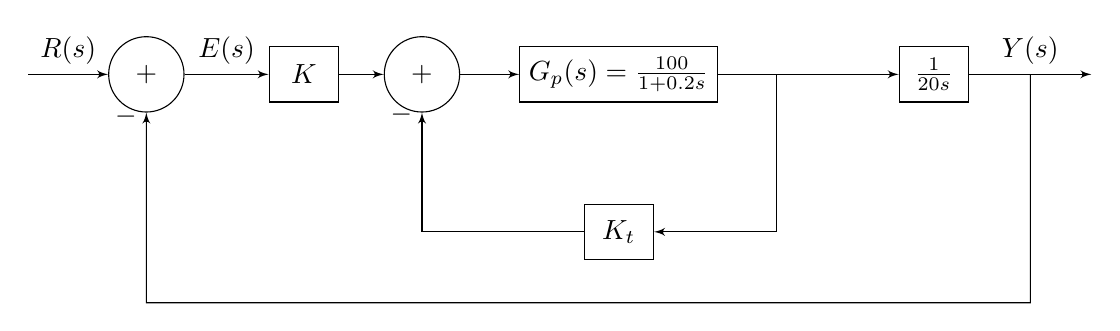
\begin{tikzpicture}[scale=0.8, auto, node distance=2cm,>=latex']
    % Drawing blocks and nodes
    \node [input, name=input] {};
    \node [sum, right of=input] (sum1) {$+$};
    \node [block, right of=sum1] (K) {$K$};
    \node [sum, right of=K] (sum2) {$+$};
    \node [block, right of=sum2, node distance=2.5cm] (Gp) {$G_p(s) = \frac{100}{1 + 0.2s}$};
    \coordinate[right of=Gp] (middle);
    \node [block, right of=middle] (sys) {$\frac{1}{20s}$};
    \node [output, right of=sys] (output) {};
    \node [block, below of=Gp] (Kt) {$K_t$};
    
    % Connectors
    \draw [draw,->] (input) -- node {$R(s)$} (sum1);
    \draw [->] (sum1) -- node {$E(s)$} (K);
    \draw [->] (K) -- node {} (sum2);
    \draw [->] (sum2) -- node {} (Gp);
    \draw [-] (Gp) -- node {} (middle);
    \draw [->] (middle) -- node {} (sys);
    \draw [->] (sys) -- node [name=Y] {$Y(s)$} (output);
    \draw [->] (middle) |- (Kt);
    \draw [->] (Kt) -| node[pos=0.99, left] {$-$} (sum2);
    \draw [->] (Y) -- ++ (0,-4) -| node[pos=0.99] {$-$} 
        node [near end] {} (sum1);
\end{tikzpicture}
\end{center}

\subsection*{Objective}
\subsubsection*{Find Steady-State Errors}
Calculate the steady-state errors for the control system, assuming it is stable. The steady-state errors should be expressed in terms of \(K\) and \(K_t\). Perform these calculations for the following input functions:

\begin{enumerate}
    \item \( r(t) = u_s(t) \)
    \item \( r(t) = tu_s(t) \)
    \item \( r(t) = \frac{t^2}{2}u_s(t) \)
\end{enumerate}

\newpage
\subsection*{Solution}
\subsubsection*{Simplify Block Diagram}
After Diagram Simplification, we are left with a Unity-feedback System, as shown below:
\begin{center}
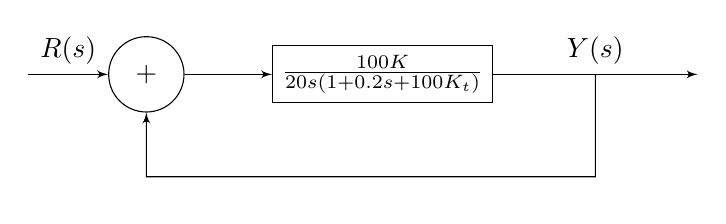
\begin{tikzpicture}[scale=0.8, auto, node distance=2cm,>=latex']
    % We start by placing the blocks
    \node [input, name=input] {};
    \node [sum, right of=input] (sum1) {$+$};
    \node [block, right of=sum1, node distance=3cm] (system) {$\frac{100K}{20s(1 + 0.2s + 100K_t)}$};
    \node [output, right of=system, node distance=4cm] (output) {};

    % Once the nodes are placed, connecting them is easy. 
    \draw [draw,->] (input) -- node {$R(s)$} (sum1);
    \draw [->] (sum1) -- node {} (system);
    \draw [->] (system) -- node [name=y] {$Y(s)$}(output);
    \draw [->] (y) -- ++(0,-2) -| node [near start, below] {} (sum1);
\end{tikzpicture}
\end{center}
\noindent
The poles of \(G(s)\) are \(0, 0, 0, -2, -2\). Three poles are at the origin, and two are negative. Therefore, the system is marginally stable.

\noindent
Given a unity feedback system with the transfer function:
\[
G(s) = \frac{100K}{20s(1 + 0.2s + 100K_t)}
\]
To calculate the steady-state errors for this system, we first need to determine the error constants for position (\(K_p\)), velocity (\(K_v\)), and acceleration (\(K_a\)). These are found using the following limits:
\begin{align*}
K_p &= \lim_{s \to 0} G(s) \\
K_v &= \lim_{s \to 0} sG(s) \\
K_a &= \lim_{s \to 0} s^2G(s)
\end{align*}
The error constants are calculated as:
\begin{align*}
K_p &= \lim_{s \to 0} \frac{100K}{20s(1 + 0.2s + 100K_t)} = \infty \\
K_v &= \lim_{s \to 0} s \left(\frac{100K}{20s(1 + 0.2s + 100K_t)}\right) = \frac{5K}{100K_t + 1} \\
K_a &= \lim_{s \to 0} s^2 \left(\frac{100K}{20s(1 + 0.2s + 100K_t)}\right) = 0
\end{align*}
Using the error constants, we can now calculate the steady-state errors for the given inputs. The steady-state error (\(e_{ss}\)) for a unity feedback system can be calculated for different types of inputs as follows:

\begin{enumerate}
    \item For a step input \( r(t) = u_s(t) \), the steady-state error is given by:
    \[
    e_{ss} = \frac{1}{1 + K_p}
    \]
    Since \( K_p = \infty \), the steady-state error \( e_{ss} \) for a step input is \( 0 \).
    
    \item For a ramp input \( r(t) = tu_s(t) \), the steady-state error is:
    \[
    e_{ss} = \frac{1}{K_v} = \frac{100K_t + 1}{5K}
    \]
    
    \item For a parabolic input \( r(t) = \frac{t^2}{2}u_s(t) \), the steady-state error is infinite since \( K_a = 0 \).
\end{enumerate}









\newpage
\section*{Problem 4}

The unit-step response of a linear control system is shown in the Figure.

\begin{figure}[h]
    \centering
    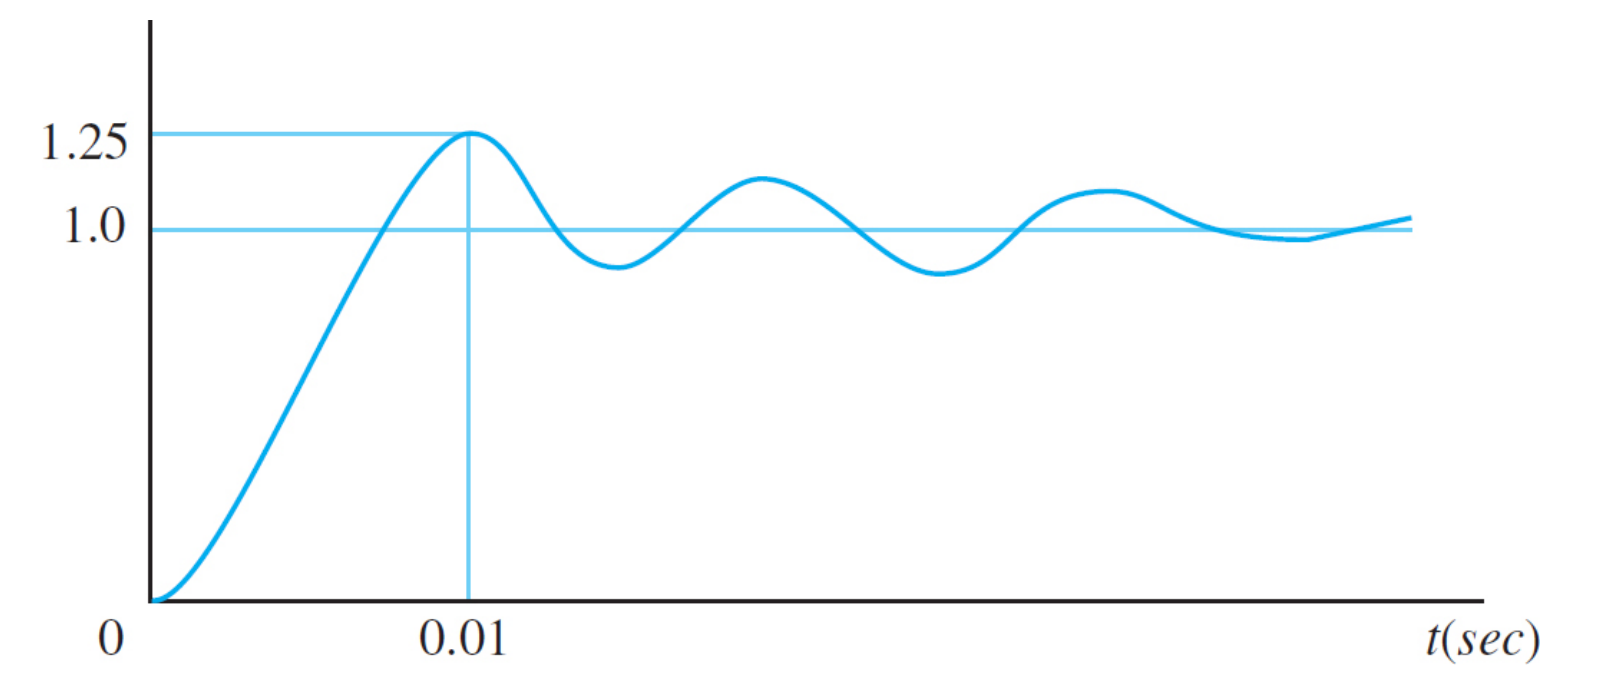
\includegraphics[width=0.8\linewidth]{Figure_P4.png} % replace 'path_to_your_figure.png' with your actual path and filename
    \caption{Unit-step response of the control system.}
    \label{fig:unit_step_response}
\end{figure}
\subsection*{Objective}
\noindent Find the transfer function of a second-order prototype system to model the system.
\newpage
\subsection*{Solution}
The observed step response indicates an overshoot, which suggests that the system can be modeled by a second-order underdamped system. The transfer function for such a system is given by:
\[
G(s) = \frac{\omega_n^2}{s^2 + 2\zeta\omega_n s + \omega_n^2}
\]
where \( \omega_n \) is the natural frequency, and \( \zeta \) is the damping ratio.

\noindent
From the given step response data, we have:
\begin{itemize}
    \item The desired output value \( D = 1 \).
    \item The peak overshoot \( M_p = 1.25 \) at time \( t_p = 0.01 \) seconds.
\end{itemize}
\noindent
The overshoot \( M_p \) is related to the damping ratio \( \zeta \) by the equation:
\[
M_p = e^{-\frac{\pi\zeta}{\sqrt{1-\zeta^2}}}
\]
Solving for \( \zeta \), we find the damping ratio to be approximately \( 0.404 \).

\noindent
The damped natural frequency \( \omega_d \) can be found from the time to the first peak \( t_p \):
\[
\omega_d = \frac{\pi}{t_p}
\]
The natural frequency \( \omega_n \) is then calculated using the damping ratio \( \zeta \) and the damped natural frequency \( \omega_d \):
\[
\omega_n = \frac{\omega_d}{\sqrt{1-\zeta^2}}
\]
This gives us \( \omega_n \) to be approximately \( 343.39 \) radians per second.

\noindent
The resulting transfer function, with the calculated parameters and rounded to decimal values, is:
\[
G(s) = \frac{117914.16}{s^2 + 277.26s + 117914.16}
\]





\newpage
\section*{Problem \#5}

A control system is shown below:
\subsection*{Block Diagram}

\begin{center}
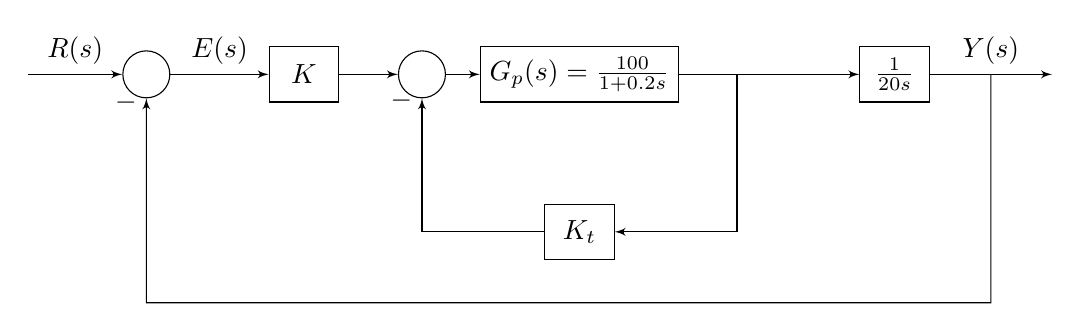
\begin{tikzpicture}[scale=0.8, auto, node distance=2cm,>=latex']
    % Drawing blocks and nodes
    \node [input, name=input] {};
    \node [sum, right of=input] (sum1) {};
    \node [block, right of=sum1] (K) {$K$};
    \node [sum, right of=K] (sum2) {};
    \node [block, right of=sum2] (Gp) {$G_p(s) = \frac{100}{1 + 0.2s}$};
    \coordinate[right of=Gp] (middle);
    \node [block, right of=middle] (sys) {$\frac{1}{20s}$};
    \node [output, right of=sys] (output) {};
    \node [block, below of=Gp] (Kt) {$K_t$};
    
    % Connectors
    \draw [draw,->] (input) -- node {$R(s)$} (sum1);
    \draw [->] (sum1) -- node {$E(s)$} (K);
    \draw [->] (K) -- node {} (sum2);
    \draw [->] (sum2) -- node {} (Gp);
    \draw [-] (Gp) -- node {} (middle);
    \draw [->] (middle) -- node {} (sys);
    \draw [->] (sys) -- node [name=Y] {$Y(s)$} (output);
    \draw [->] (middle) |- (Kt);
    \draw [->] (Kt) -| node[pos=0.99, left] {$-$} (sum2);
    \draw [->] (Y) -- ++ (0,-4) -| node[pos=0.99] {$-$} 
        node [near end] {} (sum1);
\end{tikzpicture}
\end{center}
\subsection*{Objective}
Find the values of \( K \) and \( K_t \) so that the maximum overshoot of the output is approximately \( 10\% \) and the rise time \( t_r \) is approximately \( 0.1 \, \text{s} \). Use 
\[
\omega_n \sqrt{1 - \zeta^2} t = n\pi, \quad \text{where } n = 0, 1, 2, 3, \ldots
\]
for the rise-time relationship.
\newline \newline
\noindent Simulate the system with MATLAB to check the accuracy of your solutions.
\newpage

\subsection*{Solutions}
The transfer function from the block diagram is given by:
\begin{equation*}
G(s) = \frac{Y(s)}{R(s)} = \frac{\frac{KG_2(s)}{1+KG_2(s)} + \frac{1}{s}}{1+ \frac{KG_2(s)}{1+KG_2(s)} + \frac{1}{s}}
\end{equation*}
Substituting \(G_2(s) = \frac{100}{1+0.2s}\) into the equation, we get:
\begin{align*}
G(s) &= \dfrac{\frac{K \left( \frac{100}{1+0.2s} \right)}{1+K \left( \frac{100}{1+0.2s} \right)} + \frac{1}{s}}{1 + \frac{K \left( \frac{100}{1+0.2s} \right)}{1+K \left( \frac{100}{1+0.2s} \right)} + \frac{1}{s}} \\
&= \dfrac{1}{s} + \dfrac{2000Ks + 100K}{s^2 + 20s + 2000Ks +100K} \\
&= \dfrac{4s^2 + 20s + 2000Ks +100K}{s^3 + 20s^2 + 2000Ks +100K} \\
&= \dfrac{4s^2 + (20+2000K)s +100K}{s(s^2 + 20s + 2000Ks +100K)} \\
&= \dfrac{s^2 + (5+500K)s + 25K}{s^3 + (5+500K)s^2 + 25K}
\end{align*}
The second-order prototype transfer function is:
\begin{equation*}
G(s) = \frac{\omega_n^2}{s^2 + 2\zeta\omega_n s + \omega_n^2}
\end{equation*}
Comparing the coefficients, we obtain:
\begin{align*}
\omega_n &= \sqrt{25K} \\
\zeta &= \frac{5+500K}{2\omega_n}
\end{align*}
The maximum overshoot is given by:
\begin{equation*}
\text{maximum overshoot} = e^{\frac{-\pi\zeta}{\sqrt{1-\zeta^2}}}
\end{equation*}
For a given maximum overshoot of 10\%, we find:
\begin{align*}
0.10 &= e^{\frac{-\pi\zeta}{\sqrt{1-\zeta^2}}} \\
\zeta &= \sqrt{1-\left(\frac{\ln(0.10)}{\pi}\right)^2} = 0.59
\end{align*}
The rise time is given by an expression as follows:
\begin{equation*}
t_r = \frac{1 - 0.4167 \zeta + 2.917 \zeta^2}{\omega_n}
\end{equation*}
Given the value of damping ratio \( \zeta = 0.59 \) and the rise time \( t_r = 0.1 \) s, we substitute the corresponding values into the above equation to obtain an expression for \( \omega_n \) as follows:
\begin{equation*}
0.1 = \frac{1 - 0.4167(0.59) + 2.917(0.59)^2}{\omega_n}
\end{equation*}
Simplifying the above equation gives:
\begin{equation*}
\omega_n = \frac{1 - 0.4167(0.59) + 2.917(0.59)^2}{0.1}
\end{equation*}
\begin{equation*}
\omega_n = \frac{1.7696}{0.1} = 17.7 \text{ rad/s}
\end{equation*}
Substitute the values of \(\omega_n\) and \(\zeta\) to find:
\begin{align*}
K &= \left(\frac{\omega_n}{5}\right)^2 = 12.53 \\
K_t &= \frac{2\zeta\omega_n - 5}{500} = 0.0318
\end{align*}
The final transfer function is:
\begin{equation*}
G(s) = \frac{25K}{s^3 + (5+500K_t)s^2 + 25K} = \frac{313.25}{s^3 + 20.9s^2 + 313.25}
\end{equation*}
\newpage
\subsection*{MATLAB Simulation and Verification}
Here is the MATLAB code used for the simulation:

\begin{lstlisting}[language=Matlab]
% Clear the environment and close all figure windows
clc; 
clear; 
close all;

% Transfer function coefficients
num_coeffs = [313.25];
denom_coeffs = [1, 20.9, 313.25];

% Create the transfer function for the system
sys_transfer_func = tf(num_coeffs, denom_coeffs);

% Time settings
simulation_end_time = 1; % End time for simulation in seconds
time_vec = 0:0.01:simulation_end_time; % Time vector from 0 to end_time with a step of 0.01 seconds

% Generate and plot the step response over the specified time vector
fig_handle = figure; % Create a new figure and get the handle
[step_response, time] = step(sys_transfer_func, time_vec);
step(sys_transfer_func, time_vec);
title('Step Response over 1 Second');

% Retrieve step response characteristics
step_info = stepinfo(step_response, time) % Get step info using the output data and time

% Display the graph window
shg;

% Save the figure to a file
print(fig_handle, 'StepResponsePlot', '-dpng');

\end{lstlisting}
\newpage
\subsection*{Simulation Result}
The result of the MATLAB simulation is shown in Figure \ref{fig:matlabresult}.

\begin{figure}[h]
    \centering
    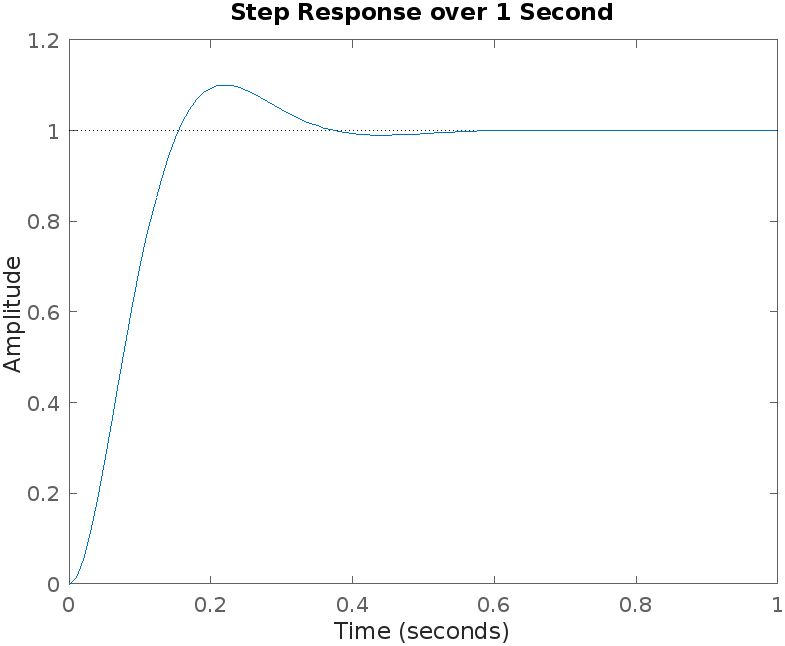
\includegraphics[width=0.75\textwidth]{export.png}
    \caption{MATLAB simulation result}
    \label{fig:matlabresult}
\end{figure}
\subsection*{MATLAB Results}
Results from the MATLAB simulation are summarized below:
\begin{itemize}
    \item Rise Time: 0.1038 seconds
    \item Transient Time: 0.3349 seconds
    \item Settling Time: 0.3349 seconds
    \item Settling Min: 0.9423
    \item Settling Max: 1.1004
    \item Overshoot: 10.0451\%
    \item Undershoot: 0
    \item Peak: 1.1004
    \item Peak Time: 0.2200 seconds
\end{itemize}




\newpage
\section*{Problem \#6}

A control system is shown below:
\subsection*{Block Diagram}

\begin{center}
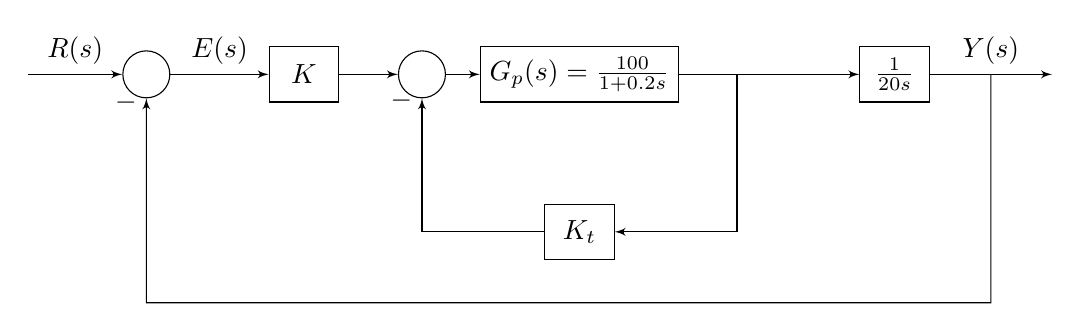
\begin{tikzpicture}[scale=0.8, auto, node distance=2cm,>=latex']
    % Drawing blocks and nodes
    \node [input, name=input] {};
    \node [sum, right of=input] (sum1) {};
    \node [block, right of=sum1] (K) {$K$};
    \node [sum, right of=K] (sum2) {};
    \node [block, right of=sum2] (Gp) {$G_p(s) = \frac{100}{1 + 0.2s}$};
    \coordinate[right of=Gp] (middle);
    \node [block, right of=middle] (sys) {$\frac{1}{20s}$};
    \node [output, right of=sys] (output) {};
    \node [block, below of=Gp] (Kt) {$K_t$};
    
    % Connectors
    \draw [draw,->] (input) -- node {$R(s)$} (sum1);
    \draw [->] (sum1) -- node {$E(s)$} (K);
    \draw [->] (K) -- node {} (sum2);
    \draw [->] (sum2) -- node {} (Gp);
    \draw [-] (Gp) -- node {} (middle);
    \draw [->] (middle) -- node {} (sys);
    \draw [->] (sys) -- node [name=Y] {$Y(s)$} (output);
    \draw [->] (middle) |- (Kt);
    \draw [->] (Kt) -| node[pos=0.99, left] {$-$} (sum2);
    \draw [->] (Y) -- ++ (0,-4) -| node[pos=0.99] {$-$} 
        node [near end] {} (sum1);
\end{tikzpicture}
\end{center}

\subsection*{Objective}
Find the values of \( K \) and \( K_t \) so that the maximum overshoot of the output is approximately \( 4.3\% \) and the delay time \( t_d \) is approximately \( 0.1 \, \text{s} \). Use 
\[
\frac{dy(t)}{dt} = \frac{\omega_n e^{-\zeta \omega_n t}}{\sqrt{1 - \zeta^2}} \left[ \zeta \sin(\omega t + \theta) - \sqrt{1 - \zeta^2} \cos(\omega t + \theta) \right], \quad \text{when } t \geq 0
\]
for the delay-time relationship.
\newline \newline
\noindent Simulate the system with MATLAB to check the accuracy of your solutions.
\newpage

The transfer function from the above mentioned block diagram can be written as follows after rearranging terms and simplifying:
\begin{equation*}
    G(s) = \frac{100}{s^2 + (5+500K_t)s + 25K}
\end{equation*}

Compare equations (1) and (2) to obtain the value of undamped natural frequency \( \omega_n \) and damping ratio \( \zeta \) as follows:
\begin{align*}
    \omega_n &= 25K \\
    2\zeta \omega_n &= 5 + 500K_t
\end{align*}

The maximum overshoot is given by:
\begin{equation*}
    \text{maximum overshoot} = e^{\left( -\frac{\pi \zeta}{\sqrt{1-\zeta^2}} \right)}
\end{equation*}
Given the value of maximum overshoot is 4.3\%, we find \( \zeta \) by substituting the overshoot value into the following equation:
\begin{equation*}
    \zeta = \sqrt{\frac{\ln^2(0.042)}{\pi^2 + \ln^2(0.042)}}
\end{equation*}
Solve the above equation to find \( \zeta \).

The delay time is given by:
\begin{equation*}
    t_d = \frac{1.1 + 0.125 \omega_n + 0.469 \zeta^2}{\omega_n}
\end{equation*}
Substitute the corresponding values to find \( t_d \).

To find the values of \( K \) and \( K_t \), we use:
\begin{align*}
    K &= \frac{\omega_n^2}{25} \\
    K_d &= \frac{2\zeta \omega_n - 5}{500}
\end{align*}

Substitute the values of \( K \) and \( K_d \) in the above equation (1) to obtain the final expression for \( G(s) \):
\begin{equation*}
    G(s) = \frac{202.5}{s^3 + 20.1s^2 + 202.5}
\end{equation*}
\newpage


\subsection*{MATLAB Simulation and Verification}
Here is the MATLAB code used for the simulation:

\begin{lstlisting}[language=Matlab]
% Clear the environment and close all figure windows
clc; 
clear; 
close all;

% Transfer function coefficients
num_coeffs = [202.5];
denom_coeffs = [1, 20.1, 202.5];

% Create the transfer function for the system
sys_transfer_func = tf(num_coeffs, denom_coeffs);

% Time settings
simulation_end_time = 1; % End time for simulation in seconds
time_vec = 0:0.01:simulation_end_time; % Time vector from 0 to end_time with a step of 0.01 seconds

% Generate and plot the step response over the specified time vector
fig_handle = figure; % Create a new figure and get the handle
[step_response, time] = step(sys_transfer_func, time_vec);
step(sys_transfer_func, time_vec);
title('Step Response over 1 Second');

% Retrieve step response characteristics
step_info = stepinfo(step_response, time) % Get step info using the output data and time

% Display the graph window
shg;

% Save the figure to a file
print(fig_handle, 'StepResponsePlot', '-dpng');

\end{lstlisting}
\newpage
\subsection*{Simulation Result}
The result of the MATLAB simulation is shown in Figure \ref{fig:matlabresult}.

\begin{figure}[h]
    \centering
    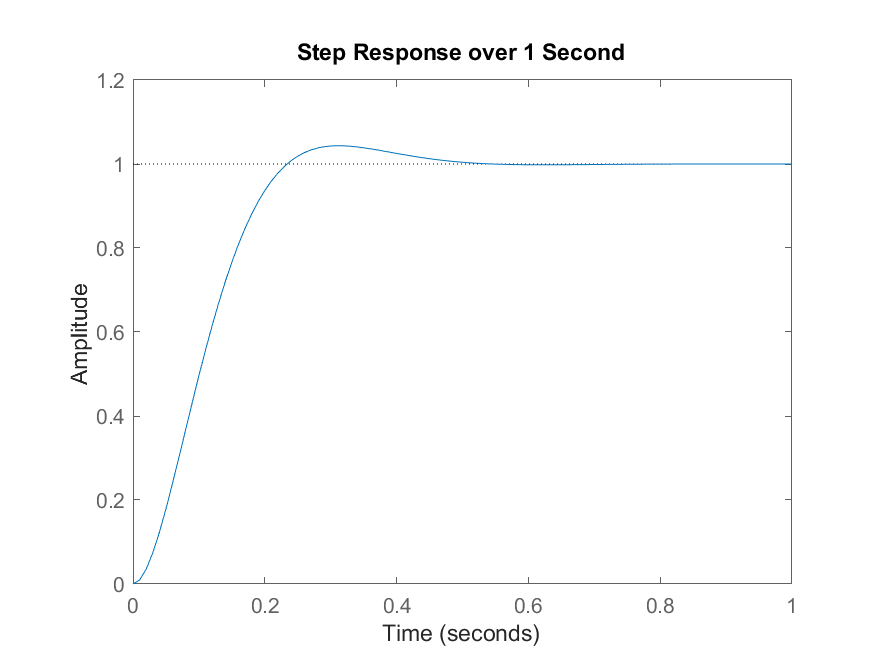
\includegraphics[width=0.75\textwidth]{StepResponsePlot2.png}
    \caption{MATLAB simulation result}
    \label{fig:matlabresult}
\end{figure}
\subsection*{MATLAB Results}
Results from the MATLAB simulation are summarized below:
\begin{itemize}
    \item Rise Time: 0.1511 seconds
    \item Transient Time: 0.4189 seconds
    \item Settling Time: 0.4189 seconds
    \item Settling Min: 0.9107
    \item Settling Max: 1.0435
    \item Overshoot: 4.3469\%
    \item Undershoot: 0
    \item Peak: 1.0435
    \item Peak Time: 0.3100 seconds
\end{itemize}

\newpage
\section*{Problem \#7}
The Figure shows the block diagram of a servomotor.
\subsection*{Block Diagram}
\begin{center}
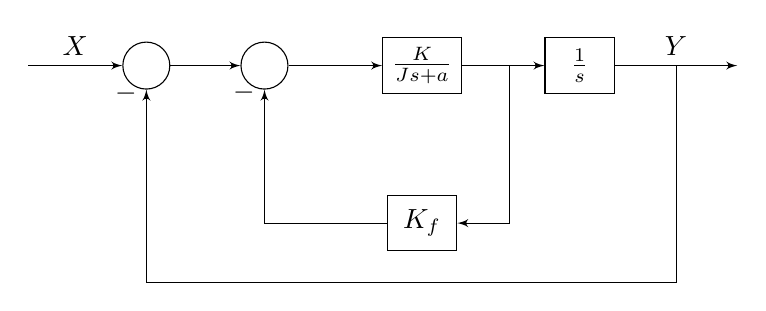
\begin{tikzpicture}[scale=1.2, auto, node distance=2cm,>=latex']
    % Define the nodes
    \node [input, name=input] {};
    \node [sum, right of= input] (sum1) {};
    \node [sum, right of= sum1] (sum2) {};
    \node [block, right of= sum2] (block1) {$\frac{K}{Js+a}$};
    \node [block, right of= block1] (block2) {$\frac{1}{s}$};
    \node [output, right of= block2] (output) {};
    \node [block, below of= block1] (block3) {$K_f$};
    % Connect the nodes
    \draw [->] (input) -- node[name=X] {$X$} (sum1);
    \draw [->] (sum1) -- (sum2);
    \draw [->] (sum2) -- (block1);
    \draw [->] (block1) -- (block2);
    \draw [->] (block2) -- node[name=Y] {$Y$} (output);
    \draw [->] (block1.east) -- ++(0.5cm,0) |- (block3);
    \draw [->] (block3) -| node[pos=0.99] {$-$} node [near end, left] {} (sum2);
    \draw [->] (Y) |- ++(0,-2.5cm) -| node[pos=0.99] {$-$} node [near end, right] {} (sum1);
\end{tikzpicture}
\end{center}
\subsection*{Objective}

\noindent Assume \( J = 1 \) kg-m\(^2\) and \( B = 1 \) N \( \cdot \) m/rad/s. If the maximum overshoot of the unit-step input and the peak time are 0.2 and 0.1 s, respectively,

\begin{enumerate}
    \item Find its damping ratio and natural frequency.
    \item Find the gain \( K \) and velocity feedback \( K_f \). Also, calculate the rise time and settling time.
\end{enumerate}

\newpage
\noindent
After rearranging the block diagram and simplifying, we arrive at a unity-feedback system with an open-loop transfer function:
\begin{equation*}
    \frac{K}{s(Js + a + KK_f)}.
\end{equation*}
Solving for the closed-loop function, we obtain:
\begin{equation*}
    \frac{K}{Js^2 + (a + KK_f)s + K}.
\end{equation*}
\newline\newline
\noindent
The damping ratio is calculated using:
\begin{equation*}
    M_p = e^{-\frac{\pi\zeta}{\sqrt{1-\zeta^2}}}.
\end{equation*}
After solving, we find that the damping ratio, \(\zeta\), is equal to 0.456.
\newline\newline
\noindent
The natural frequency is determined via:
\begin{equation*}
    t_p = \frac{\pi}{\omega_n \sqrt{1-\zeta^2}},
\end{equation*}
where \(t_p\) is the peak time. Solving for \(\omega_n\), we find that \(\omega_n\) is equivalent to 35.28 rad/sec.
\newline\newline
\noindent
Rearranging the closed-loop form of the transfer function to match the standard form, we get:
\begin{equation*}
    \frac{K/J}{s\left(s + \frac{a + KK_f}{J}\right)},
\end{equation*}
and from the standard form:
\begin{equation*}
    G(s) = \frac{\omega_n^2}{s(s + 2\zeta\omega_n)}.
\end{equation*}
From a comparison, we see that \(\omega_n = \sqrt{\frac{K}{J}}\), and solving for \(K\), we get 1244.7984.
We also see that \(2\zeta\omega_n = \frac{a + KK_f}{J}\), and solving for \(K_f\), we get 0.025.
\newline\newline
\noindent
Calculating the rise time as:
\begin{equation*}
    \frac{0.8 + 2.4\zeta}{\omega_n},
\end{equation*}
we find that \(t_r = 0.055\) seconds.
The settling time is calculated as:
\begin{equation*}
    \frac{3.2}{\omega_n\zeta} = 0.1989
\end{equation*}
seconds.


\end{document}
